\section{Google Cardboard}
%-----------------------    ---------------------------------

\begin{frame}
\frametitle{Google Cardboard}

\begin{center}
  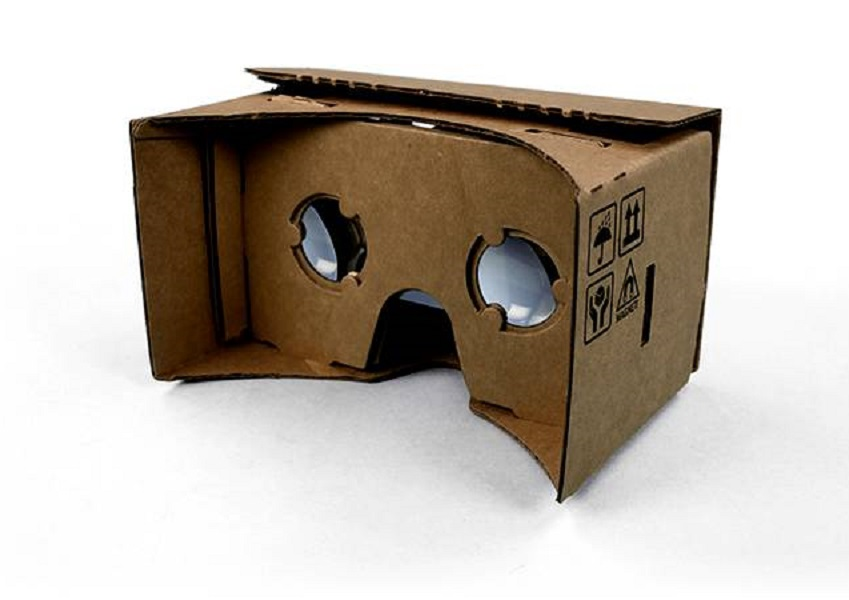
\includegraphics[width=9cm]{figs/google-cardboard.jpg}
\end{center}


\begin{flushright}
{\tiny
Source: http://images.techtimes.com/data/images/full/10137/google-cardboard.jpg
}
\end{flushright}

\end{frame}


%-----------------------    ---------------------------------

\begin{frame}
\frametitle{Google Cardboard}

\begin{center}
  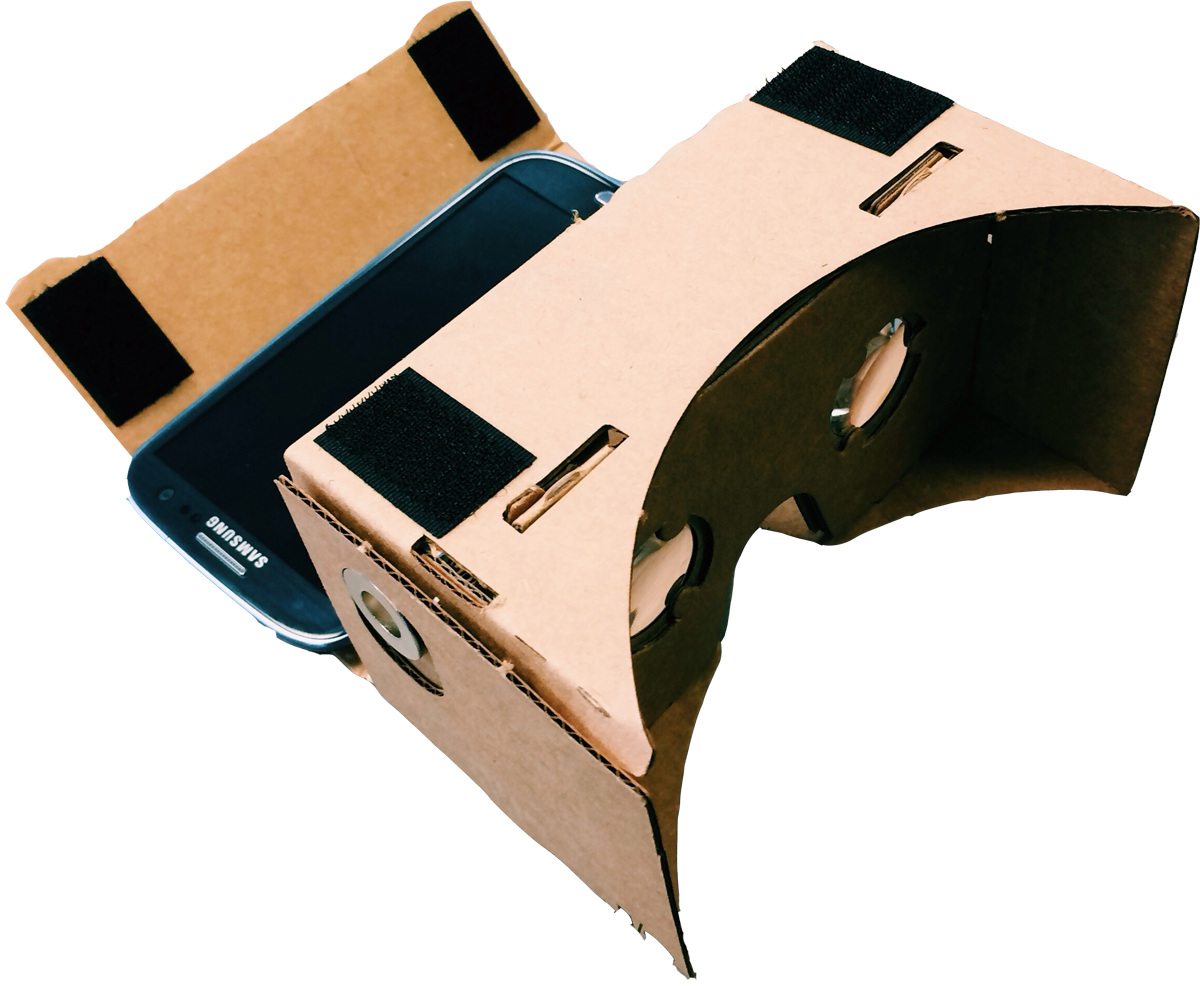
\includegraphics[width=8cm]{figs/google-cardboard2.jpg}
\end{center}


\begin{flushright}
{\tiny
Source: http://uploads.webflow.com/53acec028f16901b3d5ca6c1/53acec104f02f4e04bcd4ec5\_1.png
}
\end{flushright}

\end{frame}


%-----------------------    ---------------------------------

\begin{frame}
\frametitle{¿Qué es el Google Cardboard?}

\begin{itemize}
   \item Experimenta realidad virtual de manera sencilla y barata (19 euros)
   \item Cuesta de 2 euros (tiendas chinas on-line) a 35 euros (la ``oficial'')
   \item Aunque hay instrucciones para hacerla tú mismo con una caja de pizza)
   \item Hay varias aplicaciones en el Google Play: cardboard, etc.
   \item API en Java
   \item También se pueden utilizar extensiones de Chrome escritas en Javascript (con Tree.js)
\end{itemize}

\end{frame}


%-----------------------    ---------------------------------

\begin{frame}
\frametitle{Google Cardboard ``ingredients''}

\begin{center}
  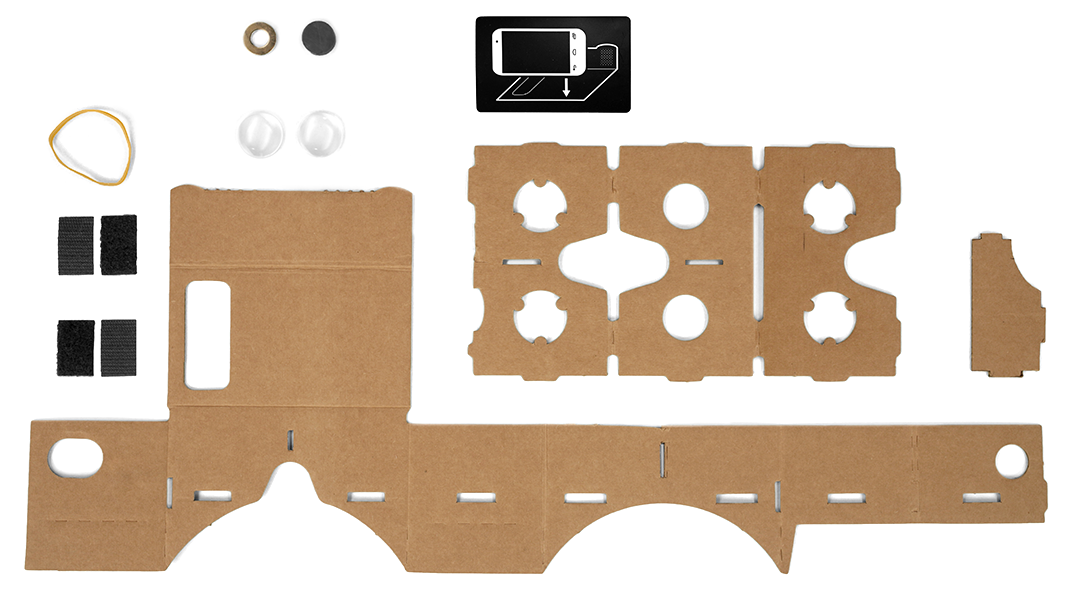
\includegraphics[width=11cm]{figs/ingredients.png}
\end{center}


\begin{flushright}
{\tiny
Source: https://cardboard.withgoogle.com/
}
\end{flushright}

\end{frame}


